\documentclass[12pt,a4paper]{article}

\usepackage[utf8]{inputenc}   % Je kunt gewóón accenten typen, als je wilt
\usepackage[T1]{fontenc}      % Nodig om de accenten ook ín de pdf te krijgen
\usepackage[english]{babel}     % Figuur i.p.v. Figure, en NL afbrekingen
\usepackage{amssymb}          % Voor extra symbolen
\usepackage{amsmath}          % Voor extra ondersteuning bij vergelijkingen (zie documentatie)
\usepackage{a4wide}           % Past marges aan voor A4.
\usepackage[small]{caption}   % Voor bijschriften met een iets kleinere lettergrootte dan de hoofdtekst.
\usepackage{url}              % Voor het beter weergeven van url's (lang, of met speciale tekens)
\usepackage{booktabs}         % Voor professionele tabellen
\usepackage[output-decimal-marker={,},list-final-separator={ en }]{siunitx}          % Voor het typesetten en uitlijnen van getallen en eenheden, zie documentatie
\usepackage[pdfusetitle]{hyperref}  % Voor handige links in je PDF. B.v. urls, referenties, etc.
\usepackage{ upgreek }
\usepackage{ dsfont }
\usepackage{mathtools}
\usepackage{ textcomp }
\linespread{1.3}

%% DOCUMENT PROPERTIES
\author{Lois de Grootte - 12136646\\
Timo van Hattum - \\
Sancho Luijten - 11700556\\
Jelmer Mulder - 12181102}
\title{How to Make an Alien on GJ 1214 b}
\date{\today}
\begin{document}

%% BEGIN TITELPAGINA
\begin{titlepage}
\maketitle
\thispagestyle{empty} % geen paginanummer op de titelpagina

\vfill
% Samenvatting
\abstract{\small ................ \\[2ex]}

 \begin{table}[h]
  \label{tab:credits}
  \begin{tabular}{l l}
   \textsc{Study}: Psychobiology and Physics \& Astronomy\\
   \textsc{Commissioned by}: How to Make an Alien \\
  \end{tabular}
  \vspace{3ex}
 \end{table}
 
\begin{figure}
  \centering  
  
\includegraphics[width=150mm]{logo-combi-vu-uva-nl}\\   % UvA logo
  \vspace{-13ex}
 \end{figure}

\end{titlepage}

\setcounter{page}{2}    
\suppressfloats[t] 
---------------------------------------------- \\

\section{Equations}
Most equations in astronomy and physics are commonly known. Here we will state all equations which we use without a derivation. For derivations, we refer to \textit{An Introduction to Astrophysics} \cite{introduction_to_astrophysics}.

\subsection*{Light}
\begin{align}
	\nonumber d(pc) &= \frac{R(\text{rad})}{p''} \\
	d(pc) &= \frac{1 (\text{AE})}{p''} \\
 	L &= 4 \pi R^2 \sigma T^4 	\label{eq:luminosity} \\
 	f &= \frac{L}{4 \pi d^2} \label{eq:flux}\\
	\nonumber m - m_0&= -2.5 \log(\frac{f}{f_0}) \\
	\nonumber M_1 - M_2 &= -2.5 \log(\frac{L_1}{L_2}) \\
	m - M &= 5 \log d - 5 \label{eq:distance_modules} \\
	I(\nu, T) &= \frac{2 h \nu^3}{c^2} \frac{1}{\exp{\frac{h \nu}{k T} - 1}} \label{eq:planck_light}\\
	\lambda_{\text{max}}  T &= b = 2.9*10^{-3} \label{eq:Wien}
\end{align}

\subsection*{Gravity}
\begin{align}
    F &= \frac{m v^2}{r} \\
	v &= \sqrt[2]{\frac{G M}{r}} \label{eq:middelpuntzoekendekracht} \\
	F_{1,2} &= G \frac{m_1 M_2}{r^2} \label{eq:gravity}
\end{align}

\subsection*{Kepler}
\begin{align}
    r(\phi) &= \frac{a (1-e^2}{(1 - e) \cos(\phi)} \\
	O &= \pi a b = \pi a^2 \sqrt[2]{1 - e^2} \\
	\frac{P^2}{r^3} &= \frac{4 \pi^2}{G (M + m)} \approx \frac{4 \pi^2}{G M}
\end{align}
\newpage
\section{All parameters}
\subsection{Gliese 1214}
\begin{table}[]
\centering
\caption{}
\label{tab:star-char}
\begin{tabular}{l|l}
Parameter    & Units                               \\ \hline
Distance     & 14.55(13) pc \cite{Anglada_2013}    \\
Stellar Mass & 0.157 M                             \\
Radius       & 0.201(10) R \cite{Anglada_2013}     \\
Luminosity   & $4.05(19) * 10^{-3}$ L \cite{Anglada_2013} \\
Temperature  & 3252(20) K \cite{Anglada_2013}      \\
Wavelength peak   & $9.68 * 10^{-7}$ m      
\end{tabular}
\end{table}

\subsection{Gliese 1214b}
\begin{table}[]
\centering
\caption{}
\label{tab:planet-char}
\begin{tabular}{l|l}
\textbf{Parameter} & \textbf{Units}                     \\ \hline
Mass               & 6.55(98) M                         \\
Radius             & 2.678(130) R                       \\
Period             & 1.5803952(137) day                 \\
Density            & 1870(400) kg m$^{-3}$              \\
Orbital Radius     & 0.01438(19) AU                     
\end{tabular}
\end{table}

\subsubsection{Equilibrium Temperature}
We can calculate the equilibrium temperature by 
\begin{equation}
    E_{\text{in}} = E_{\text{out}},
\end{equation}
where $E_{\text{in}}$ depends on the albedo, flux and radius of the planet and $E_{\text{out}}$ is just the luminosity of the planet. Substituting eq. (\ref{eq:luminosity}) and (\ref{eq:flux}) gives,
\begin{align}
    \text{Albedo} * \text{Flux} * \text{Area of incident} &= L_{\text{planet}} \\
    (1 - \alpha) \frac{L_{\text{star}}}{4 \pi d^2} \pi R_{\text{planet}}^2 &= 4 \pi R_{\text{planet}}^2 \sigma T_{\text{planet}}^4 \\
    T_{\text{planet}}^4 &= \frac{L_{\text{star}} (1 - \alpha)}{16 \pi d^2 \sigma},
\end{align}
where $d$ is the orbital distance, $\sigma$ is the Stefan-Boltzmann constant and $T_{\text{planet}}$ is the final equilibrium temperature. We can simplify this equation by substituting \ref{eq:luminosity},
\begin{equation}
    T_{\text{planet}} = \sqrt[4]{\frac{R_{\text{star}}^2 T_{\text{star}}^4}{4 d^2} (1 - \alpha)}.
\end{equation}
%Temprature calculation
By substituting the known parameters from \ref{tab:planet-char}, we can calculate its equilibrium temperature. The albedo is unknown, so we will calculate both limits, with an albedo of $\alpha = 0.75$  for its minimal temperature and $\alpha = 0$ for its maximum temperature.
\begin{align*}
    T_{\text{min}} &= \sqrt[4]{\frac{(0.201 R_{\text{Sun}})^2 3252^4}{4 (0.01438 1.49 10^11)} (1 - 0.75)} = 415 K \\
    T_{\text{max}} &= \sqrt[4]{(\frac{0.201 R_{\text{Sun}})^2 3252^4}{4 (0.01438 1.49 10^{11})} (1 - 0)} = 588 K.
\end{align*}
These limits are a good approximation because we know GJ 1214b is not a Neptune-planet, which has an albedo of $\alpha = 0.75$.

\subsection{Atmosphere}
A study from 2009 concluded that the atmosphere from Gliese 1214b evaporates. However, due to a constant supply of material from its surface, it still holds a atmosphere, a non-primordal atmosphere\cite{Charbonneau_2009}. So if this planet contains life, it should not be carried away by the evaporation.
In the same study, they compared Gliese 1214b with mass-radius models of rocky, water and gaseous planets \cite{Charbonneau_2009}. They concluded it is probably a water-dominated planet, with a gaseous atmosphere surrounding it. If this is indeed is the case, the extreme atmosferic pressure and the lack-of solar radiation, will hinder life development. However, a study from 2010 looked at three different cases:  \cite{Rogers_2010}

%Three cases: H2/He accretion, ice-rocky, rock-evaporation.

\section{Energy}
The exact type of atmosphere of GJ 1214b is unknown. The energy distribution of a planet depends on different factors, like albedo, cloud coverage, humidity and atmosphere. Some are unknown while others have been measured. Here we will unravel these unknown aspects of GJ 1214b and make some calculations and assumptions considering <case 2?>. \\
In a study from 2014, partially written by Jean-Michel Désert, they studied recent transmission spectra of GJ 1214b made by the Hubble Space Telescope. They only found featureless spectra, which means cloud-free atmosphere containing water, methane and carbon-dioxide where ruled out. They concluded the planet needs to have some sort of cloud layer to match the obtained data \cite{Kreidberg_2014}. Because there is no data that can be used to determine the type of clouds, we can not make any assumptions about the role of clouds in the temperature of GJ 1214b. Higher clouds will increase green-house effects while lower thickers clouds will increase a planets albedo \cite{SteveGrahamClouds}. \\
Considering <case2?>, live can only exist in higher parts of the atmosphere. So without studying the conditions at lower altitudes where they may even be water plasma \cite{Rogers_2010}, a few assumptions can be made. The ocean planet GJ 1214b will have a water dominated atmosphere. The humidity will thus be very high and the green-house effect needs to be taken into account for the energy-budget of this planet. \\
Taking the above into consideration, a rough estimate of the albedo can be made. An albedo of $\alpha = 0.4(2)$ will be reasonable.  
\subsection{Radiation spectrum of GJ 1214}
The star Gliese 1214 is a red M-dwarf with a mass of 0.157 M. Gliese 1214 radiates infrared light with a luminosity 0.33 per cent that of the sun which is 4.05(19)*10-3 L \cite{Anglada_2013}. To measure the radiation spectrum of GJ 1214 the effective temperature and the radii must be determined. As shown in \textit{table 1} the Teff = 3252 K and R = 0.201 (10) R. A reliable mechanism to determine the spectral energy distribution is through photometry \cite{Anglada_2013}. In our case it’s a infrared photometry. 

Researchers in article \cite{Anglada_2013} measured the radiation spectrum of GJ 1214 in different effective temperatures and radii as shown in \textit{figure 1}. The best fit for GJ 1214 is the green spectral template with Teff = 3250 K and R = 0.20 Rsun \cite{Anglada_2013}. It shows that the wavelength peak is 9.68*10-7 m. 

\textit{Figure 2} shows the electromagnetic spectrum. Visible light has a lower wavelength than infrared. The wavelength peak on earth is 550 nm which corresponds with green light. Photosynthesis on earth happens in green plants by chlorophyll. Plants absorb blue and red light very well, therefore chlorophyll reflects green light \cite{ijms15034657} and that’s why the plants on earth are green. 

If the energy of the radiation of GJ 1214 is used for life on GJ 1214b like on earth, it would be most efficient to have red plants. The color red has a wavelength around 700 nm, which is the nearest color to the wavelength peak of the radiation coming from GJ 1214. 
On the other hand, it could be possible that the plants on GJ 1214b do not have a visible color but absorbs and reflects different wavelength of infrared light. 

\begin{figure}
  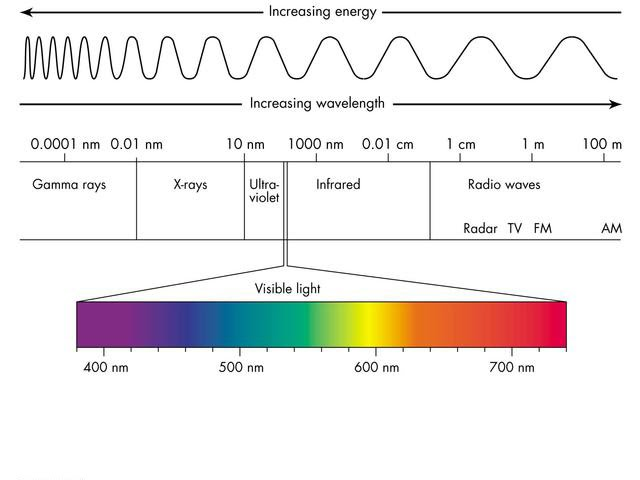
\includegraphics[width=100mm]{EMSpectrumcolor.jpg}\\   
  \vspace{-13ex}
  \label{fig:Electromagnetic spectrum}
 \end{figure}



\bibliographystyle{science}
\bibliography{bronnen}
\end{document}

